\documentclass[11pt,a4paper,oneside]{report}
\usepackage{amsmath,amssymb,calc,ifthen}
\usepackage{float}
%\usepackage{cancel}
\usepackage[table,usenames,dvipsnames]{xcolor} % for coloured cells in tables
\usepackage{tikz}
% Allows us to click on links and references!
\usepackage{hyperref}
\usepackage{url}
\hypersetup{
colorlinks,
citecolor=black,
filecolor=black,
linkcolor=black,
urlcolor=black
}
% Nice package for plotting graphs
% See excellent guide:
% http://www.tug.org/TUGboat/tb31-1/tb97wright-pgfplots.pdf
\usetikzlibrary{plotmarks,shapes}
\usepackage{amsmath,graphicx}
\usepackage{epstopdf}
\usepackage{caption}
\usepackage{subcaption}
% highlight - useful for TODOs and similar
\usepackage{color}
\newcommand{\hilight}[1]{\colorbox{yellow}{#1}}
\newcommand\ci{\perp\!\!\!\perp} % perpendicular sign
\newcommand*\rfrac[2]{{}^{#1}\!/_{#2}} % diagonal fraction
\newcommand\SLASH{\char`\\}
\usepackage{listings}
% margin size
\usepackage[margin=0.65in]{geometry}

\usepackage{titlesec} % reduce spacing after subsections

\titlespacing\subsection{0pt}{4pt plus 4pt minus 2pt}{4pt plus 2pt minus 2pt}

\usepackage{multicol}

\tikzstyle{state}=[circle,thick,draw=black, align=center, minimum size=2.1cm,
inner sep=0]
\tikzstyle{vertex}=[circle,thick,draw=black]
\tikzstyle{terminal}=[rectangle,thick,draw=black]
\tikzstyle{edge} = [draw,thick]
\tikzstyle{lo} = [edge,dotted]
\tikzstyle{hi} = [edge]
\tikzstyle{trans} = [edge,->]
\definecolor{mygreen}{rgb}{0,0.6,0}
\definecolor{mygray}{rgb}{0.5,0.5,0.5}
\definecolor{mymauve}{rgb}{0.58,0,0.82}
\DeclareMathOperator*{\argmin}{arg\,min}
\DeclareMathOperator*{\argmax}{arg\,max}
\lstset{ %
backgroundcolor=\color{white}, % choose the background color; you must add
%\usepackage{color} or \usepackage{xcolor}
basicstyle=\footnotesize, % the size of the fonts that are used for the
%code
breakatwhitespace=false, % sets if automatic breaks should only happen
%at whitespace
breaklines=true, % sets automatic line breaking
captionpos=b, % sets the caption-position to bottom
commentstyle=\color{mygreen}, % comment style
deletekeywords={...}, % if you want to delete keywords from the
%given language
escapeinside={\%*}{*)}, % if you want to add LaTeX within your code
extendedchars=true, % lets you use non-ASCII characters; for
%8-bits encodings only, does not work with UTF-8
frame=single, % adds a frame around the code
keepspaces=true, % keeps spaces in text, useful for keeping
%indentation of code (possibly needs columns=flexible)
keywordstyle=\color{blue}, % keyword style
language=Octave, % the language of the code
morekeywords={*,...}, % if you want to add more keywords to the set
numbers=left, % where to put the line-numbers; possible
%values are (none, left, right)
numbersep=5pt, % how far the line-numbers are from the code
numberstyle=\tiny\color{mygray}, % the style that is used for the line-numbers
rulecolor=\color{black}, % if not set, the frame-color may be changed
%on line-breaks within not-black text (e.g. comments (green here))
showspaces=false, % show spaces everywhere adding particular
%underscores; it overrides 'showstringspaces'
showstringspaces=false, % underline spaces within strings only
showtabs=false, % show tabs within strings adding particular
%underscores
stepnumber=2, % the step between two line-numbers. If it's
%1, each line will be numbered
stringstyle=\color{mymauve}, % string literal style
tabsize=2, % sets default tabsize to 2 spaces
title=\lstname % show the filename of files included with
%\lstinputlisting; also try caption instead of title
}
\title{Computational Modelling for Biomedical Imaging - Individual Report}
\author{
Razvan Valentin Marinescu\\
Student Number: 14060166\\
\texttt{razvan.marinescu.14@ucl.ac.uk}
}



\begin{document}
\belowdisplayskip=12pt plus 3pt minus 9pt
\belowdisplayshortskip=7pt plus 3pt minus 4pt

\begin{titlepage}
\begin{center}

% Upper part of the page. The '~' is needed because \\
% only works if a paragraph has started.

\includegraphics[width=0.2\textwidth]{ucl-logo2}~\\[1cm]

\textsc{\LARGE University College London}\\[1.5cm]

\newcommand{\HRule}{\rule{\linewidth}{0.5mm}}

% Title
\HRule \\[0.4cm]
{ \Large Information Processing in Medical Imaging - Coursework Report \\[0.4cm] }

\HRule \\[1.5cm]

% Author and supervisor
\begin{minipage}{0.4\textwidth}
% \begin{flushleft} \large
\centering
\emph{Author:}\\
R\u{a}zvan Valentin \textsc{Marinescu}\\
\href{razvan.marinescu.14@ucl.ac.uk}{razvan.marinescu.14@ucl.ac.uk}\\
% \end{flushleft}
\end{minipage}


\vfill

\vfill
\vfill

EPSRC Centre for Doctoral Training in Medical Imaging\\ University College London

\vfill

% Bottom of the page
{\large \today}

\end{center}
\end{titlepage}


%\maketitle{}



% \rowcolors{2}{gray!25}{white}

\section*{Task I - Full brain segmentation}

\subsection*{Proposed pipeline}

Segmentation propagation (\texttt{p1reg.py}) has been performed on the extra 5 AD and 5 controls, both baseline and followup images, using the tutorial instructions from the CMIC TIG website. This means that we needed to propagate segmentations for 20 different images, and since we had 10 source templates available, this meant 200 propagations. As each propagation took around 1.5 minutes on an Intel(R) Xeon(R) CPU @ 3.60GHz, a careful balance between computation time and accuracy had to be obtained. The parameters chosen were: 
\begin{itemize}
 \item \texttt{reg\_aladin}: --speeeed (parameter that speeded up the affine registration)
 \item \texttt{reg\_f3d}: number of levels: 4, number of iterations: 200
\end{itemize}
A discussion about how I chose these parameters is given at the end of this section. After performing the 

% TODO add the plots with parameters choices and dice scores

\subsection*{Parameters}

\section*{Task II - Atrophy measurement}

The BSI has been computed using the method described in Leung et al. \cite{leung2010robust}. First, the baseline and followup images have been aligned using the 9DOF affine registration. Then, the union and intersection regions of the images is computed. The union is dilated once, while the intersection is eroded once using a structure that looks like a 3x3x3 sphere. The brain boundary shift region is then given by the XOR of the dilated union and eroded intersection. 
The intensity of both images is then normalised by dividing by the mean intensity inside the intersect region. Finally, the BSI is computed using a manually chosen intensity window of [0.45,0.65] recommended by Freeborough and Fox, 1997. \cite{freeborough1997boundary}.

\begin{figure}[H]
 \centering
 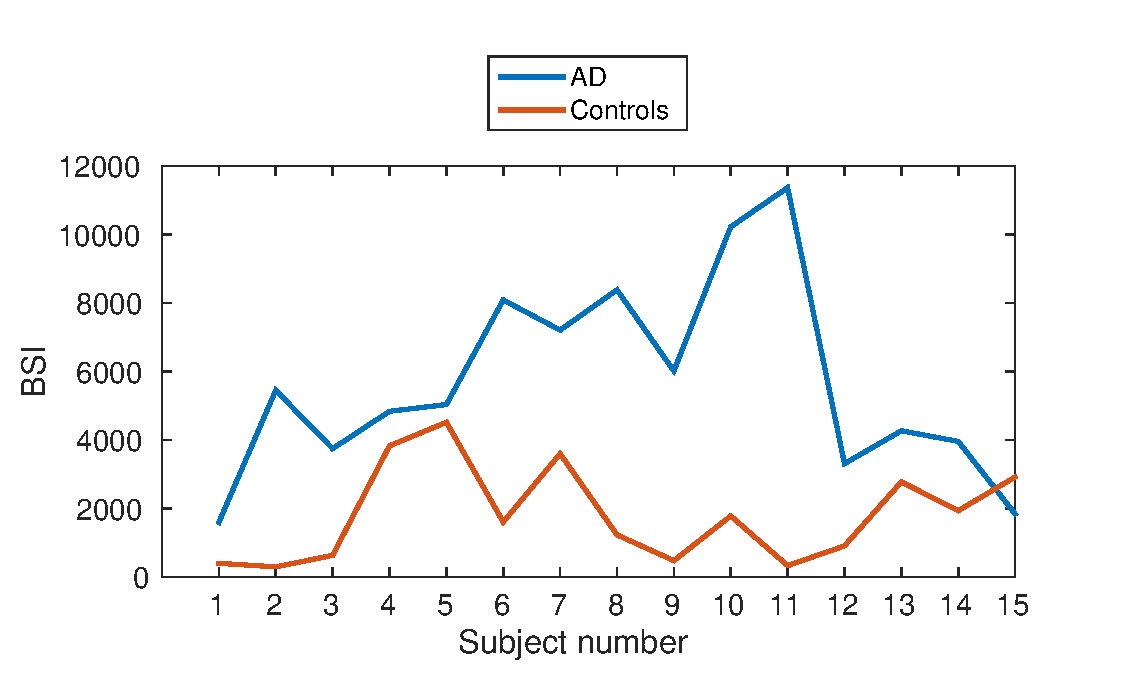
\includegraphics[scale=0.7]{figures/bsi_plot.eps}
 \caption{BSI measurements for all AD and control subjects. Each AD patient is paired with an age-matched control, typically a spouse or carer. \cite{malone2013miriad} There is visibly more atrophy (as measured by BSI) for AD subjects compared to control subjects. The only exception is subject 15, which might be an outlier.}
\end{figure}

\begin{figure}[H]
 \centering
 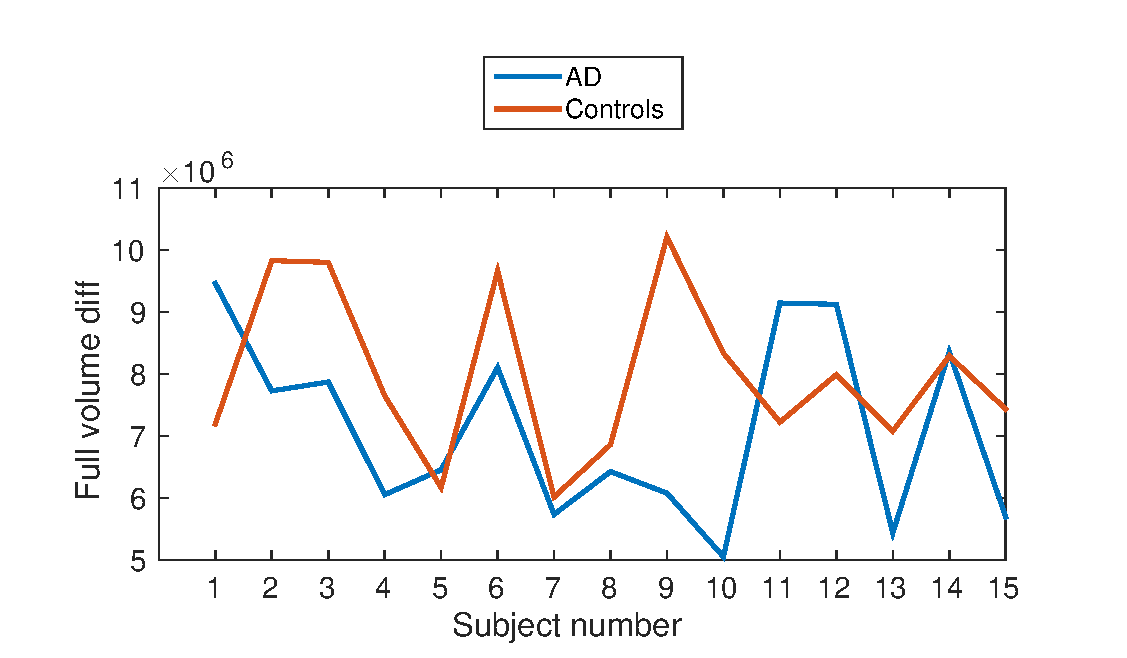
\includegraphics[scale=0.7]{figures/fullVolumePlot.eps}
 \caption{Full volume difference for all AD and control subjects. There is considerable more overlap between AD and controls }
\end{figure}



\section*{Task III - Statistical Analysis}

\subsection*{T-tests}

A two-sample t-test has been performed for AD and control groups using the BSI, in order to see if there is a statistically significant difference in atrophy. Since each AD patient had an age-matched control (normally a spouse or carer ) \cite{malone2013miriad}, this allows us to also perform a paired t-test, checking for a pairwise difference in atrophy. A similar analysis has been made using the full-volume difference. Results are presented in the following table:\\

\begin{center}
 \begin{tabular}{c | c | c | c | c}
 Metric & \multicolumn{2}{c|}{paired-sample t-test} & \multicolumn{2}{c}{two-sample t-test}\\  
 & $H_0$ & p-value & $H_0$ & p-value\\
 \hline
 BSI & \cellcolor{green!15} rejected & 5.23e-04& \cellcolor{green!15}rejected & 6.45e-05\\
 Full-volume & \cellcolor{red!15} not rejected & 0.0844 & \cellcolor{red!15} not rejected & 0.1062\\
 
 \end{tabular}
\end{center}

For the BSI metric, both t-tests rejected the null hypothesis $H_0$, while for the full-volume metric, $H_0$ could not be rejected. We therefore conclude that there is a significant difference of atrophy between AD and control groups, as measured by the BSI. Furthermore, we also conclude that BSI is better than the full-volume difference at discriminating between AD and control subjects. 

\subsection*{Sample size analysis}

MATLAB function \texttt{samplesizepwr} has been used to calculate the sample size required to detect a 25\% atrophy rate with an 80\% power (file \texttt{p3.m}). For the BSI, minimum sample sizes of 34 and 77 are required to detect an atrophy reduction relative to AD and normal ageing respectively. Similarly, for the Full brain volume, minimum sample sizes of 8 and 6 are required to detect an atrophy reduction relative to AD and normal ageing, respectively. The reason for the lower sample size required using the full volume atrophy is because the standard deviation of the groups was much lower relative to the mean.

% sample_size 34, 77, 8, 6


\subsection*{Future improvements}


\bibliographystyle{plain}
\bibliography{citations}

\end{document}





















